\subsection{ADPLL - digital, discretized PLL Model}\label{adpll_model}
Based on the continuous PLL theory, a model for digital, discrete time sampled PLLs (i.e. ADPLLs) can be adapted. The general approach here is to utilize the bilinear transformation between continuous s-domain models to the discrete z-domain models and vice-versa. As commonly cited in PLL literature from a seminal paper by Gardner \cite{gardner_1980}, if the PLL sampling frequency $f_s > 10\cdot\textnormal{BW}_{loop}$, where BW$_{loop}$ is the PLL loop bandwidth, the granularity effects due to time-sampling can be neglected. Thus the design methods established in this paper are predicated on $f_s > 10\cdot\textnormal{BW}_{loop}$.
\begin{figure}[htb!]
	\center\fontfamily{\sfdefault}\selectfont
% XCircuit output "basic_adpll.tex" for LaTeX input from basic_adpll.ps
\def\putbox#1#2#3#4{\makebox[0.00000in][l]{\makebox[#1][l]{}\raisebox{\baselineskip}[0.00000in][0.00000in]{\raisebox{#2}[0.00000in][0.00000in]{\scalebox{#3}{#4}}}}}
\def\rightbox#1{\makebox[0.00000in][r]{#1}}
\def\centbox#1{\makebox[0.00000in]{#1}}
\def\topbox#1{\raisebox{-0.60\baselineskip}[0.00000in][0.00000in]{#1}}
\def\midbox#1{\raisebox{-0.20\baselineskip}[0.00000in][0.00000in]{#1}}
   \scalebox{1}{
   \normalsize
   \parbox{5.07500in}{
   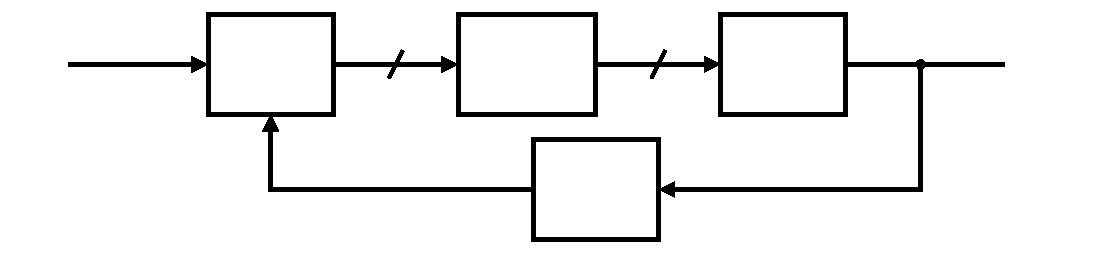
\includegraphics[scale=0.70000]{./figs/basic_adpll.pdf}\\
   % translate x=368 y=488 scale 0.38
   \putbox{1.09200in}{0.82600in}{1.20}{TDC}%
   \putbox{2.63200in}{0.24500in}{1.20}{$\div$ N}%
   \putbox{0.35700in}{0.97300in}{1.20}{$\Phi_{ref}$[n]}%
   \putbox{4.09500in}{0.97300in}{1.20}{$\Phi_{out}$[n]}%
   \putbox{2.19800in}{0.82600in}{1.20}{H$_{LF}$(z)}%
   \putbox{3.47900in}{0.82600in}{1.20}{DCO}%
   \putbox{1.67300in}{0.39200in}{1.20}{$\Phi_{div}$[n]}%
   \putbox{1.64500in}{1.02900in}{1.20}{e$_{\Phi}$[n]}%
   \putbox{2.92600in}{1.02900in}{1.20}{u[n]}%
   } % close 'parbox'
   } % close 'scalebox'
   \vspace{-\baselineskip} % this is not necessary, but looks better
\fontfamily{\rmdefault}\selectfont

	\caption{Basic ADPLL.}
	\label{fig:basic_adpll}
\end{figure}
\FloatBarrier
The basic architecture of an ADPLL is shown in figure \ref{fig:basic_adpll}. Here, compared to the continuous PLL of figure \ref{fig:basic_pll}, the phase detector has been replaced with a time to digital converter (TDC), the loop filter $\mathrm{H}_{LF}(s)$ with a discrete-time loop filter $\mathrm{H}_{LF}(z)$, and the VCO with a digitally controlled oscillator (DCO). In this architecture, all components are fully or partially digital in implementation. 

\subsubsection{Divider}\label{div_theory}
	A digital divider functions by counting input cycles. With a divider modulus N, the output of the divider will have an active edge transition (considered to be rising edge as shown in figure \ref{fig:digital_div}) every N-cycles. Phase information is inferred from active edge timing, which occurs with time interval N$/f_{osc}$, and is equal to the point at which output phase equals a multiple of $2\pi$. Thus a digital divider does not provider continuous phase information, but rather a sampled phase signal with rate $f_{osc}/$N. 
	\begin{figure}[htb!]
		\center\fontfamily{\sfdefault}\selectfont
% XCircuit output "digital_div.tex" for LaTeX input from digital_div.ps
\def\putbox#1#2#3#4{\makebox[0.00000in][l]{\makebox[#1][l]{}\raisebox{\baselineskip}[0.00000in][0.00000in]{\raisebox{#2}[0.00000in][0.00000in]{\scalebox{#3}{#4}}}}}
\def\rightbox#1{\makebox[0.00000in][r]{#1}}
\def\centbox#1{\makebox[0.00000in]{#1}}
\def\topbox#1{\raisebox{-0.60\baselineskip}[0.00000in][0.00000in]{#1}}
\def\midbox#1{\raisebox{-0.20\baselineskip}[0.00000in][0.00000in]{#1}}
   \scalebox{1}{
   \normalsize
   \parbox{3.15000in}{
   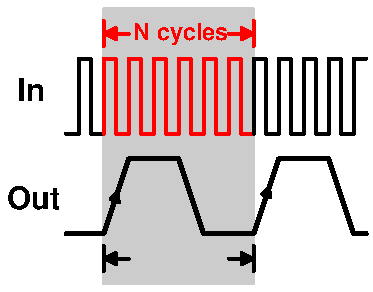
\includegraphics[scale=0.90000]{./figs/digital_div.pdf}\\
   % translate x=-16 y=516 scale 0.38
   \putbox{1.30500in}{0.16200in}{1.20}{$\mathrm{N}/f_{osc}$}%
   } % close 'parbox'
   } % close 'scalebox'
   \vspace{-\baselineskip} % this is not necessary, but looks better
\fontfamily{\rmdefault}\selectfont

		\caption{Digital divider signals.}
		\label{fig:digital_div}
	\end{figure}

	For PLL transfer function modeling, a digital divider behaves identically to the continuous case:
	\begin{equation}
		\Phi_{div}[n] = \frac{\Phi_{out}[n]}{\mathrm{N}}
	\end{equation}
	Application of the z- and s-domain transformations:
	\begin{equation}
		\mathrm{H}_{div}(z) = \mathrm{H}_{div}(s) = \frac{\Phi_{div}(z)}{\Phi_{out}(z)} = \frac{1}{\mathrm{N}}
	\end{equation}

\subsubsection{TDC}
	The TDC is a digital, quantized representation of the phase detector. It takes input phase signals $\Phi_{div}$[n] and $\Phi_{ref}$[n], and outputs a digital phase error word $e_\Phi[n]$. Figure \ref{fig:tdc} shows the basic TDC model architecture. Being digitized, a TDC will have limited resolution in phase, equivalent to M steps per reference cycle. This is a minimum step size in time of $\Delta t_{step}$ = $1/Mf_{ref}$. Since the output of the TDC is digital, the model applies a scale factor M$/2\pi$ and floor rounding, so 1 least significant bit (LSB) of $e_\Phi[n]$ equates to $\Delta t_{step}$ timing error  between $\Phi_{div}$[n] and $\Phi_{ref}$[n].
	\begin{figure}[htb!]
		\center\fontfamily{\sfdefault}\selectfont
% XCircuit output "tdc.tex" for LaTeX input from tdc.ps
\def\putbox#1#2#3#4{\makebox[0.00000in][l]{\makebox[#1][l]{}\raisebox{\baselineskip}[0.00000in][0.00000in]{\raisebox{#2}[0.00000in][0.00000in]{\scalebox{#3}{#4}}}}}
\def\rightbox#1{\makebox[0.00000in][r]{#1}}
\def\centbox#1{\makebox[0.00000in]{#1}}
\def\topbox#1{\raisebox{-0.60\baselineskip}[0.00000in][0.00000in]{#1}}
\def\midbox#1{\raisebox{-0.20\baselineskip}[0.00000in][0.00000in]{#1}}
   \scalebox{1}{
   \normalsize
   \parbox{3.50000in}{
   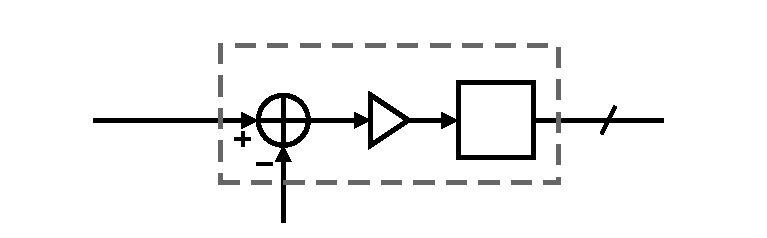
\includegraphics[scale=0.70000]{./figs/tdc.pdf}\\
   % translate x=432 y=396 scale 0.38
   \putbox{0.46200in}{0.63700in}{1.20}{$\Phi_{ref}$[n]}%
   \putbox{1.35100in}{0.08400in}{1.20}{$\Phi_{div}$[n]}%
   \putbox{2.68100in}{0.66500in}{1.20}{e$_\Phi$[n]}%
   \putbox{1.77800in}{0.70700in}{1.20}{\rotatebox{-360}{$\frac{\mathrm{M}}{2\pi}$}}%
   \putbox{1.47000in}{0.63700in}{1.20}{$\Phi_e$}%
   \putbox{2.18400in}{0.50400in}{1.20}{$\lfloor x\rfloor$}%
   \putbox{1.02900in}{0.95900in}{1.20}{TDC}%
   } % close 'parbox'
   } % close 'scalebox'
   \vspace{-\baselineskip} % this is not necessary, but looks better
\fontfamily{\rmdefault}\selectfont

		\caption{TDC model.}
		\label{fig:tdc}
	\end{figure}
	\FloatBarrier
	In sampled-time equation form:
	\begin{equation}
		e_\Phi[n] = \left\lfloor\frac{\mathrm{M}}{2\pi}(\Phi_{ref}[n] - \Phi_{div}[n])\right\rfloor
	\end{equation}
	For purposes of PLL loop gain calculation, the TDC z- and s-domain representation is equation \ref{eq:tdc_tf}, which accounts for phase-to-digital domain conversion gain. Effects of quantization will be handled in section \ref{pn_theory}.
	\begin{equation}
		e_\Phi(z) = \frac{\mathrm{M}}{2\pi}(\Phi_{ref}(z) - \Phi_{div}(z))
	\end{equation}	
	\begin{equation}\label{eq:tdc_tf}
		\mathrm{H}_{TDC}(z) = \mathrm{H}_{TDC}(s) = \frac{\mathrm{M}}{2\pi}
	\end{equation}	
	\FloatBarrier

\subsubsection{Discrete-time loop filter}\label{lf-discretization}
	The discrete-time loop filter design will be derived from the continuous canonical loop filter (equation \ref{eq:lf_general_form}) via application of a s-to-z domain transformation. The bilinear transform \cite{proakis_1993_bilinear} allows for such conversion from continuous transfer function to discrete representation. However, in the case presented in this work, where a high degree of sampling ($f_s > 10\cdot\mathrm{BW}_{loop}$) is employed, a simpler transformation is permissible, derived through Taylor series approximation of z=$re^{s\Delta T}$ for values on the unit circle, i.e. r=1. This will be referred to as the approximate bilinear transform in this work. Given the $1/\Delta T_s$=$f_{ref}$ as the relation for sampling rate, then:
	\begin{align*}
		z^{-1} &= e^{-s\Delta T_s} && \text{(definition of z-space on unit circle)} \\
		&= \sum_{k=0}^\infty\frac{(-s\Delta T_s)^k}{k!} && \text{(exponential Taylor series)} \\
		&\approx 1-s\Delta T_s &&\text{(if $|s\Delta T_s| = 2\pi\mathrm{BW}_{loop}\cdot \Delta T_s << 1$)} \\
	\end{align*}
	Thus the s-to-z and z-to-s identities for the approximated bilinear transform are:
	\begin{align}
		z^{-1} &= 1-s\Delta T_s\\
		s &= \frac{1}{\Delta T_s}(1-z^{-1}) \label{eq:s_to_z_xfrm}
	\end{align}
	Applying \ref{eq:s_to_z_xfrm} to equation \ref{eq:lf_general_form} yields the z-domain loop filter:
	\begin{align}
		\textnormal{H}_{LF}(z) &= \left.\textnormal{H}_{LF}(s)\right\vert_{s=\frac{1}{\Delta T_s}(1-z^{-1})} = \left.\frac{\sum_{j=0}^Z b_js^j}{\sum_{k=0}^P a_ks^k}\right\vert_{s=\frac{1}{\Delta T_s}(1-z^{-1})}\\
		&= \frac{\sum_{j=0}^Z b_j(1-z^{-1})^j}{\sum_{k=0}^P a_k(1-z^{-1})^k} \label{eq:z_general_lf}
	\end{align}
	Equation \ref{eq:z_general_lf} is transformed to a digitally implementable representation by reorganizing into the canonical representation of \ref{eq:canonical_z_tf}, which then determines the tap coefficients for the sampled-time difference equation \ref{eq:cananical_diff_eq}. 
	\begin{align}
		\textnormal{H}_{LF}(z) &= \frac{\sum_{j=0}^P b_j^{'}z^{-j}}{1+\sum_{k=1}^Z a_k^{'}z^{-k}}\label{eq:canonical_z_tf} \\
		y[n]&= -\sum_{k=1}^P a_k^{'}y[n-k] + \sum_{j=0}^Z b_j^{'}x[n-j] \label{eq:cananical_diff_eq}
	\end{align}
	The obtained difference equation is directly implementable in digital hardware with a direct from I IIR filter \cite{proakis_1993} shown in figure \ref{fig:filt_implementation}. The filter coefficients $\{a_1^{'}, ..., a_P^{'}\}$ and $\{b_0^{'}, ..., b_Z^{'}\}$ must be quantized into finite resolution fixed point words for a complete digital implementation. The delay elements ($z^{-1}$ blocks) are implementable digitally as registers, the coefficient gains are implementable with array multipliers and the adders are implementable with digital adders. Effects of quantization will be discussed in section \ref{pn_theory}.
	\begin{figure}[htb!]
		\center\fontfamily{\sfdefault}\selectfont
% XCircuit output "direct_type_1_primed.tex" for LaTeX input from direct_type_1_primed.ps
\def\putbox#1#2#3#4{\makebox[0.00000in][l]{\makebox[#1][l]{}\raisebox{\baselineskip}[0.00000in][0.00000in]{\raisebox{#2}[0.00000in][0.00000in]{\scalebox{#3}{#4}}}}}
\def\rightbox#1{\makebox[0.00000in][r]{#1}}
\def\centbox#1{\makebox[0.00000in]{#1}}
\def\topbox#1{\raisebox{-0.60\baselineskip}[0.00000in][0.00000in]{#1}}
\def\midbox#1{\raisebox{-0.20\baselineskip}[0.00000in][0.00000in]{#1}}
   \scalebox{1}{
   \normalsize
   \parbox{2.75990in}{
   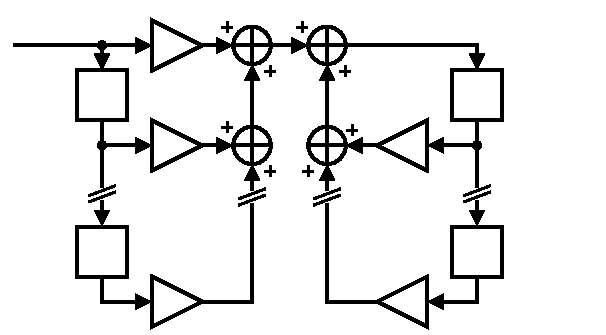
\includegraphics[scale=0.70000]{./figs/direct_type_1_primed.pdf}\\
   % translate x=936 y=992 scale 0.38
   \putbox{0.04200in}{1.42800in}{0.96}{x[n]}%
   \putbox{2.28200in}{1.33700in}{0.96}{y[n]}%
   \putbox{0.37800in}{1.07800in}{0.96}{$z^{-1}$}%
   \putbox{0.84000in}{1.45600in}{0.96}{b$_0^{'}$}%
   \putbox{0.84000in}{0.98700in}{0.96}{b$_1^{'}$}%
   \putbox{2.12800in}{1.07800in}{0.96}{$z^{-1}$}%
   \putbox{2.12800in}{0.34300in}{0.96}{$z^{-1}$}%
   \putbox{1.71500in}{1.00100in}{0.96}{-a$_1^{'}$}%
   \putbox{1.70100in}{0.27300in}{0.96}{-a$_\mathrm{P}^{'}$}%
   \putbox{2.28200in}{0.86800in}{0.96}{y[n-1]}%
   \putbox{0.37800in}{0.34300in}{0.96}{$z^{-1}$}%
   \putbox{0.84000in}{0.25900in}{0.96}{b$_\mathrm{Z}^{'}$}%
   } % close 'parbox'
   } % close 'scalebox'
   \vspace{-\baselineskip} % this is not necessary, but looks better
\fontfamily{\rmdefault}\selectfont

		\caption{Direct form I implementation of IIR filter.}
		\label{fig:filt_implementation}
	\end{figure}


\subsubsection{DCO}
	The digitally controlled oscillator varies from a VCO by only accepting a digital frequency tuning signal, called the oscillator tuning word (OTW). A DCO modeled in discrete time as a recursive phase integrator, dependent on (a) the DCO gain $K_{DCO}$, equal to the frequency tuning of the oscillator per LSB of the OTW, (b) the current state of the OTW u[n], and (c) the PLL sampling period T=$f_{ref}^{-1}$.
	\begin{equation}
		\Phi_{out}[n] = \Phi_{out}[n-1] + 2\pi K_{DCO}u[n]\Delta T_s
	\end{equation}
	Application of the z-transform yields equation \ref{eq:hdcoz}, and successive application of the bilinear transform to the DCO transfer function yields  \ref{eq:hdcos}.
	\begin{equation}\label{eq:hdcoz}
		\mathrm{H}_{DCO}(z) = \frac{\Phi_{out}(z)}{u(z)} = \frac{2\pi K_{DCO}\Delta T_s}{1-z^{-1}}
	\end{equation}
	\begin{equation}\label{eq:hdcos}
		\mathrm{H}_{DCO}(s) = \frac{\Phi_{out}(s)}{u(s)} = \frac{2\pi K_{DCO}\Delta T_s}{1-(1-s\Delta T_s)} = \frac{2\pi K_{DCO}}{s} 
	\end{equation}

\subsubsection{Discrete-time PLL transfer function}\label{discrete_pll_tf}
	\begin{figure}[htb!]
		\center\fontfamily{\sfdefault}\selectfont
% XCircuit output "discrete_pll.tex" for LaTeX input from discrete_pll.ps
\def\putbox#1#2#3#4{\makebox[0.00000in][l]{\makebox[#1][l]{}\raisebox{\baselineskip}[0.00000in][0.00000in]{\raisebox{#2}[0.00000in][0.00000in]{\scalebox{#3}{#4}}}}}
\def\rightbox#1{\makebox[0.00000in][r]{#1}}
\def\centbox#1{\makebox[0.00000in]{#1}}
\def\topbox#1{\raisebox{-0.60\baselineskip}[0.00000in][0.00000in]{#1}}
\def\midbox#1{\raisebox{-0.20\baselineskip}[0.00000in][0.00000in]{#1}}
   \scalebox{1}{
   \normalsize
   \parbox{6.88333in}{
   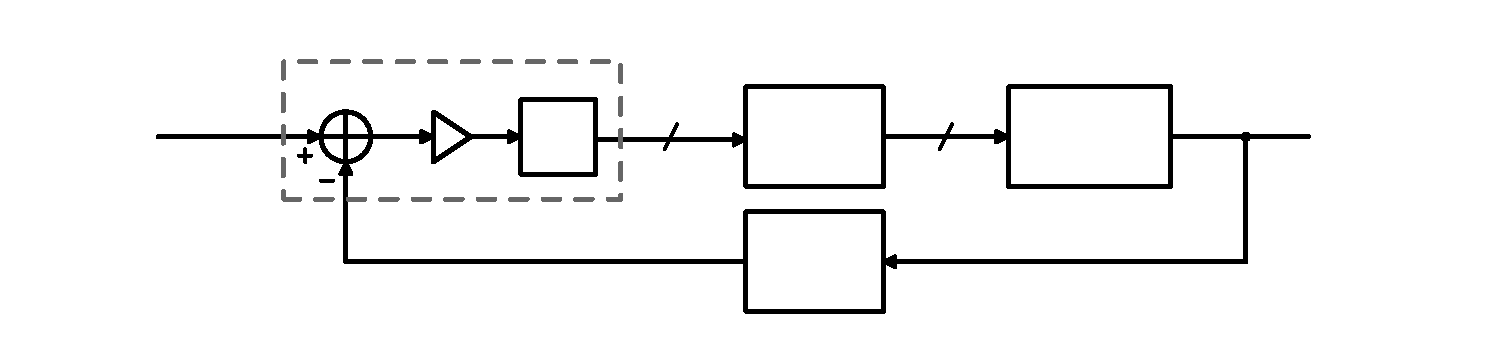
\includegraphics[scale=0.70000]{./figs/discrete_pll.pdf}\\
   % translate x=512 y=508 scale 0.38
   \putbox{0.74200in}{1.04300in}{1.20}{$\Phi_{ref}$[n]}%
   \putbox{2.17000in}{0.47600in}{1.20}{$\Phi_{div}$[n]}%
   \putbox{3.00300in}{1.07800in}{1.20}{e$_\Phi$[n]}%
   \putbox{2.06500in}{1.12000in}{1.20}{\rotatebox{-360}{$\frac{\mathrm{M}}{2\pi}$}}%
   \putbox{1.75700in}{1.04300in}{1.20}{$\Phi_e$}%
   \putbox{2.47800in}{0.91700in}{1.20}{$\lfloor x\rfloor$}%
   \putbox{1.32300in}{1.36500in}{0.90}{TDC}%
   \putbox{3.55600in}{0.91700in}{1.20}{H$_{LF}$(z)}%
   \putbox{4.28400in}{1.07800in}{1.20}{u[n]}%
   \putbox{4.73200in}{0.93100in}{1.20}{$\frac{2\pi K_{DCO}T}{1-z^{-1}}$}%
   \putbox{5.55100in}{1.04300in}{1.20}{$\Phi_{out}$[n]}%
   \putbox{3.62600in}{0.32900in}{1.20}{$\div$ N}%
   \putbox{4.70400in}{1.23200in}{0.90}{DCO}%
   } % close 'parbox'
   } % close 'scalebox'
   \vspace{-\baselineskip} % this is not necessary, but looks better
\fontfamily{\rmdefault}\selectfont

		\caption{Discrete time PLL model.}
		\label{fig:discrete_pll2}
	\end{figure}
	The transfer function for the discrete-time PLL of figure \ref{fig:discrete_pll2} can be computed in the z-domain, and also approximated continuously. The open loop z-domain transfer function is:
	\begin{align}
		\mathrm{L}(z) &= \mathrm{H}_{TDC}(z)\mathrm{H}_{LF}(z)\mathrm{H}_{DCO}(z)\mathrm{H}_{DIV}(z)
		= \frac{\mathrm{M}}{\mathrm{N}}\frac{K_{DCO}\Delta T_s}{(1-z^{-1})}\frac{\sum_{j=0}^Z b_j(1-z^{-1})^j}{\sum_{k=0}^P a_k(1-z^{-1})^k}\label{eq:z_open_loop}
	\end{align}
	The closed loop z-domain PLL phase transfer function is:
	\begin{align}
		\mathrm{T}(z) = \frac{\Phi_{out}(z)}{\Phi_{ref}(z)} &= \frac{\mathrm{M}K_{DCO}\Delta T_s\sum_{j=0}^Z b_j(1-z^{-1})^j}{\sum_{k=0}^P a_k(1-z^{-1})^{k+1} + K_{DCO}\Delta T_s\frac{\mathrm{M}}{\mathrm{N}}\sum_{j=0}^Z b_j(1-z^{-1})^j}%\\
		%&= \mathrm{N}\frac{\mathrm{L}(z)}{1+\mathrm{L}(z)}\\
	\end{align}
	The s-domain approximation of the transfer function is:
	\begin{align}
		\mathrm{L}(s) = \mathrm{H}_{TDC}(s)\mathrm{H}_{LF}(s)\mathrm{H}_{DCO}(s)\mathrm{H}_{DIV}(s) = \frac{\mathrm{M}}{\mathrm{N}}\frac{K_{DCO}}{s} \frac{\sum_{j=0}^Z b_js^j}{\sum_{k=0}^P a_ks^k}
	\end{align}
	And in closed loop configuration the s-domain PLL phase transfer function is:
	\begin{align}
		\mathrm{T}(s)=\frac{\Phi_{out}(s)}{\Phi_{ref}(s)} = \frac{\mathrm{M}K_{DCO}\sum_{j=0}^Z b_js^j}{\sum_{k=0}^P a_ks^{k+1}1 + \frac{\mathrm{M}}{\mathrm{N}}K_{DCO}\sum_{j=0}^Z b_js^j} = \mathrm{N}\frac{\mathrm{L}(s)}{1+\mathrm{L}(s)}
	\end{align}

%%%%%%%%%%%%%%%%%%%%%%%%%%%%%%%%%%%%%%%%%%%%%%%%%%%%%%%%%%%%%%%%%%%%%%%%%%%%%%%%
%%%%%%%%%%%%%%%%%%%%%%%%%%%%%%%%%%%%%%%%%%%%%%%%%%%%%%%%%%%%%%%%%%%%%%%%%%%%%%%%
% Noise
%%%%%%%%%%%%%%%%%%%%%%%%%%%%%%%%%%%%%%%%%%%%%%%%%%%%%%%%%%%%%%%%%%%%%%%%%%%%%%%%
%%%%%%%%%%%%%%%%%%%%%%%%%%%%%%%%%%%%%%%%%%%%%%%%%%%%%%%%%%%%%%%%%%%%%%%%%%%%%%%%

\subsection{ADPLL Noise Model} \label{pn_theory}
The noise in the discrete-time ADPLL result from quantization and from stochastic sources. Quantization results from round off errors introduced in the digitization of PLL components (in the TDC, loop filter, and DCO). Stochastic noise results from thermal and flicker noise in the PLL components when considered in an analog viewpoint (present in the DCO, divider and TDC). The noise generated by these quantization sources will be discussed in the following sections, based on a modeling and noise analysis approach from \cite{perrott_2002}.

\subsubsection{TDC noise}\label{tdc_noise}
	The predominant phase noise source in the TDC is due to quantization. A straightforward approach to model quantization noise is to utilize the model of figure \ref{fig:tdc_add_pn} to represent quantization.
	\begin{figure}[htb!]
	    \centering
	    \begin{subfigure}{0.5\textwidth}
	        \centering
	        \fontfamily{\sfdefault}\selectfont
% XCircuit output "tdc.tex" for LaTeX input from tdc.ps
\def\putbox#1#2#3#4{\makebox[0.00000in][l]{\makebox[#1][l]{}\raisebox{\baselineskip}[0.00000in][0.00000in]{\raisebox{#2}[0.00000in][0.00000in]{\scalebox{#3}{#4}}}}}
\def\rightbox#1{\makebox[0.00000in][r]{#1}}
\def\centbox#1{\makebox[0.00000in]{#1}}
\def\topbox#1{\raisebox{-0.60\baselineskip}[0.00000in][0.00000in]{#1}}
\def\midbox#1{\raisebox{-0.20\baselineskip}[0.00000in][0.00000in]{#1}}
   \scalebox{1}{
   \normalsize
   \parbox{3.50000in}{
   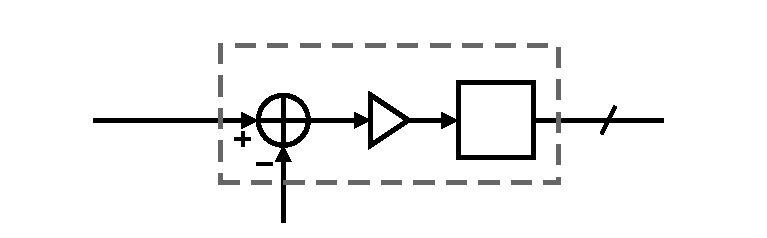
\includegraphics[scale=0.70000]{./figs/tdc.pdf}\\
   % translate x=432 y=396 scale 0.38
   \putbox{0.46200in}{0.63700in}{1.20}{$\Phi_{ref}$[n]}%
   \putbox{1.35100in}{0.08400in}{1.20}{$\Phi_{div}$[n]}%
   \putbox{2.68100in}{0.66500in}{1.20}{e$_\Phi$[n]}%
   \putbox{1.77800in}{0.70700in}{1.20}{\rotatebox{-360}{$\frac{\mathrm{M}}{2\pi}$}}%
   \putbox{1.47000in}{0.63700in}{1.20}{$\Phi_e$}%
   \putbox{2.18400in}{0.50400in}{1.20}{$\lfloor x\rfloor$}%
   \putbox{1.02900in}{0.95900in}{1.20}{TDC}%
   } % close 'parbox'
   } % close 'scalebox'
   \vspace{-\baselineskip} % this is not necessary, but looks better
\fontfamily{\rmdefault}\selectfont

	        \caption{TDC Model.}
	        \label{fig:tdc1}
	    \end{subfigure}%
	    \begin{subfigure}{0.5\textwidth}
	        \centering
	        \fontfamily{\sfdefault}\selectfont
% XCircuit output "tdc_quant.tex" for LaTeX input from tdc_quant.ps
\def\putbox#1#2#3#4{\makebox[0.00000in][l]{\makebox[#1][l]{}\raisebox{\baselineskip}[0.00000in][0.00000in]{\raisebox{#2}[0.00000in][0.00000in]{\scalebox{#3}{#4}}}}}
\def\rightbox#1{\makebox[0.00000in][r]{#1}}
\def\centbox#1{\makebox[0.00000in]{#1}}
\def\topbox#1{\raisebox{-0.60\baselineskip}[0.00000in][0.00000in]{#1}}
\def\midbox#1{\raisebox{-0.20\baselineskip}[0.00000in][0.00000in]{#1}}
   \scalebox{1}{
   \normalsize
   \parbox{3.50000in}{
   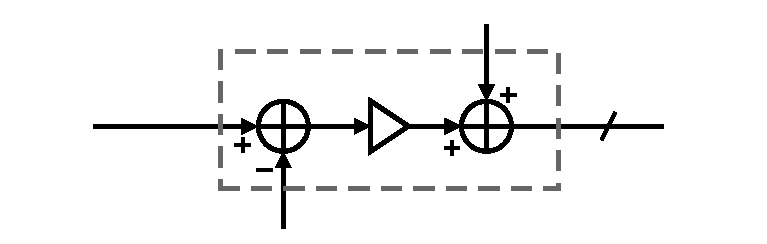
\includegraphics[scale=0.70000]{./figs/tdc_quant.pdf}\\
   % translate x=432 y=396 scale 0.38
   \putbox{0.46200in}{0.63700in}{1.20}{$\Phi_{ref}$[n]}%
   \putbox{1.35100in}{0.08400in}{1.20}{$\Phi_{div}$[n]}%
   \putbox{2.68100in}{0.66500in}{1.20}{e$_\Phi$[n]}%
   \putbox{1.77800in}{0.70700in}{1.20}{\rotatebox{-360}{$\frac{\mathrm{M}}{2\pi}$}}%
   \putbox{1.47000in}{0.63700in}{1.20}{$\Phi_e$}%
   \putbox{2.31700in}{0.97300in}{1.20}{q$_{TDC}$[n]}%
   \putbox{1.02900in}{0.95900in}{1.20}{TDC}%
   } % close 'parbox'
   } % close 'scalebox'
   \vspace{-\baselineskip} % this is not necessary, but looks better
\fontfamily{\rmdefault}\selectfont

	        \caption{TDC additive noise model.}
	        \label{fig:tdc_add_pn}
	    \end{subfigure}
	    % \caption{Approximate model for ring oscillator inverter delay cell.}
	    \label{fig:tdc_pn_model}
	    \caption{TDC quantization noise models.}
	\end{figure}
	\FloatBarrier
	Using this model, the quantized signal $e_\Phi$[n] is the sum of the its unquantized representation $\Phi_e\frac{\mathrm{M}}{2\pi}$ with a quantization error signal $\mathrm{q}_{TDC}[n]$. Figure \ref{fig:quantization} illustrates this process.
	\begin{figure}[htb!]
		\center\fontfamily{\sfdefault}\selectfont
% XCircuit output "quantization.tex" for LaTeX input from quantization.ps
\def\putbox#1#2#3#4{\makebox[0.00000in][l]{\makebox[#1][l]{}\raisebox{\baselineskip}[0.00000in][0.00000in]{\raisebox{#2}[0.00000in][0.00000in]{\scalebox{#3}{#4}}}}}
\def\rightbox#1{\makebox[0.00000in][r]{#1}}
\def\centbox#1{\makebox[0.00000in]{#1}}
\def\topbox#1{\raisebox{-0.60\baselineskip}[0.00000in][0.00000in]{#1}}
\def\midbox#1{\raisebox{-0.20\baselineskip}[0.00000in][0.00000in]{#1}}
   \scalebox{1}{
   \normalsize
   \parbox{4.24010in}{
   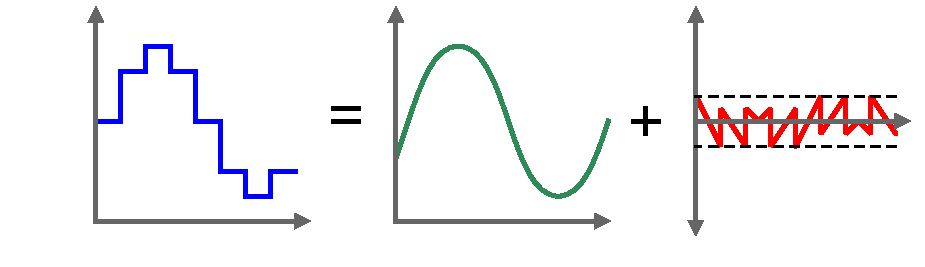
\includegraphics[scale=0.70000]{./figs/quantization.pdf}\\
   % translate x=304 y=240 scale 0.38
   \putbox{0.04200in}{1.09200in}{0.96}{$e_\Phi$[n]}%
   \putbox{1.32300in}{0.04200in}{0.96}{t=nT}%
   \putbox{1.32300in}{1.09200in}{0.96}{$\frac{\mathrm{M}}{2\pi}\Phi_e$[n]}%
   \putbox{2.77900in}{0.04200in}{0.96}{\rotatebox{-360}{t}}%
   \putbox{4.24200in}{0.50400in}{0.96}{t}%
   \putbox{2.72300in}{1.09200in}{0.96}{q$_{\mathrm{TDC}}$[n]}%
   \putbox{3.47900in}{0.85400in}{0.96}{$+\Delta/2$}%
   \putbox{3.47900in}{0.44800in}{0.96}{$-\Delta/2$}%
   } % close 'parbox'
   } % close 'scalebox'
   \vspace{-\baselineskip} % this is not necessary, but looks better
\fontfamily{\rmdefault}\selectfont

		\caption{Quantization as via additive error signal.}
		\label{fig:quantization}
	\end{figure}
	\FloatBarrier
	The quantization noise signal has the statistical property that it is uniformly distributed in the range $[-\Delta/2, \Delta/2]$, i.e. $P_q(Q=q) =\mathrm{U}(-\Delta/2, \Delta/2)$ if $\Delta$ is the quantization step size. The power of the TDC quantization noise signal is:
	\begin{equation}\label{eq:tdc_noise}
		\sigma_{q_{TDC}}^2 = \int_{-\infty}^\infty q^2P_q(Q=q)dq =  \int_{-\Delta/2}^{\Delta/2}\frac{q^2}{\Delta}dq = \frac{\Delta^2}{12}
	\end{equation}
	Since $e_\Phi$[n] is a digital signal, the minimum step size is $\Delta$=1 LSB. The TDC quantization noise power is therefore $\sigma_{q_{TDC}}^2 = 1/12$ LSB$^2$. The po
	If the quantization noise is assumed to be white, and the TDC is sampled at $f_{ref}$, the quantization PSD is:
	\begin{equation}
		S_{qn_{TDC}}(f) = \frac{P_{q_{TDC}}}{\Delta f} = \frac{\sigma_{q_{TDC}}^2}{f_{ref}} = \frac{\Delta^2}{12f_{ref}} = \frac{1}{12f_{ref}} \hspace{1em}\frac{[\text{LSB}]^2}{[\text{Hz}]}
	\end{equation}

\subsubsection{DCO noise}\label{dco_noise}
	Noise in a DCO is resulting from (a) quantization of the oscillator tuning word u[n], and (b) from thermal and stochastic sources. In the digital PLL, the OTW quantization occurs in the loop filter, so this will be analyzed in the later loop filter section (\ref{lf_noise}). Thus oscillator thermal/stochastic noise will be considered, based on Leeson's model for oscillator phase noise \cite{leeson_1966}. Leeson's model considers noise power density at an offset $\Delta f$ from the oscillator tone (carrier). Noise power density is represented with the function $\mathcal{L}(\Delta f)$, which is the noise power density normalized to the power of the oscillator carrier tone, in other words in units of dBc/Hz. Leeson's model divides phase noise into three regions, illustrated in figure \ref{fig:leeson_pn}: (1) flicker-noise dominated, with a slope of -30 dB/decade, (2) white frequency-noise dominated, with -20 dB per decade, and (3) a flat region, limited by the thermal noise floor or amplitude noise. It is noted that phase noise components are at frequencies different than the carrier, hence are orthogonal, and can be treated as independent components that are added to the main carrier frequency for analysis. Figure \ref{fig:dco_noise} demonstrates the application of this principle for modeling of the DCO phase noise $\Phi_{n_{DCO}}$ as an additive process to the oscillator phase $\Phi_{osc}$, thus $\Phi_{out}$ = $\Phi_{osc}$ + $\Phi_{n_{DCO}}$.


	\begin{figure}[htb!]
	    \centering
	    \begin{subfigure}{0.45\textwidth}
	        \centering
			\fontfamily{\sfdefault}\selectfont
% XCircuit output "leeson_pn.tex" for LaTeX input from leeson_pn.ps
\def\putbox#1#2#3#4{\makebox[0.00000in][l]{\makebox[#1][l]{}\raisebox{\baselineskip}[0.00000in][0.00000in]{\raisebox{#2}[0.00000in][0.00000in]{\scalebox{#3}{#4}}}}}
\def\rightbox#1{\makebox[0.00000in][r]{#1}}
\def\centbox#1{\makebox[0.00000in]{#1}}
\def\topbox#1{\raisebox{-0.60\baselineskip}[0.00000in][0.00000in]{#1}}
\def\midbox#1{\raisebox{-0.20\baselineskip}[0.00000in][0.00000in]{#1}}
   \scalebox{1}{
   \normalsize
   \parbox{2.68750in}{
   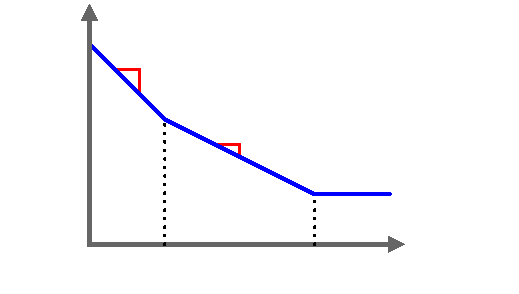
\includegraphics[scale=0.80000]{./figs/leeson_pn.pdf}\\
   % translate x=-248 y=245 scale 0.38
   \putbox{1.88000in}{0.06400in}{0.90}{$\log(\Delta f)$}%
   \putbox{0.80800in}{1.23200in}{0.72}{-30 dB/dec}%
   \putbox{0.80800in}{1.09600in}{0.72}{$\propto f^{-3}$}%
   \putbox{1.34400in}{0.73600in}{0.72}{$\propto f^{-2}$}%
   \putbox{1.34400in}{0.86400in}{0.72}{-20 dB/dec}%
   \putbox{0.80800in}{0.13600in}{0.72}{\rotatebox{-360}{$f_1$}}%
   \putbox{1.60800in}{0.13600in}{0.72}{\rotatebox{-360}{$f_2$}}%
   \putbox{0.04800in}{1.40000in}{0.90}{$\mathcal{L}(\Delta f)$}%
   } % close 'parbox'
   } % close 'scalebox'
   \vspace{-\baselineskip} % this is not necessary, but looks better
\fontfamily{\rmdefault}\selectfont

			\caption{ }
			\label{fig:leeson_pn}
	    \end{subfigure}
	    \begin{subfigure}{0.5\textwidth}
	        \centering
			\fontfamily{\sfdefault}\selectfont
% XCircuit output "dco_noise.tex" for LaTeX input from dco_noise.ps
\def\putbox#1#2#3#4{\makebox[0.00000in][l]{\makebox[#1][l]{}\raisebox{\baselineskip}[0.00000in][0.00000in]{\raisebox{#2}[0.00000in][0.00000in]{\scalebox{#3}{#4}}}}}
\def\rightbox#1{\makebox[0.00000in][r]{#1}}
\def\centbox#1{\makebox[0.00000in]{#1}}
\def\topbox#1{\raisebox{-0.60\baselineskip}[0.00000in][0.00000in]{#1}}
\def\midbox#1{\raisebox{-0.20\baselineskip}[0.00000in][0.00000in]{#1}}
   \scalebox{1}{
   \normalsize
   \parbox{3.56562in}{
   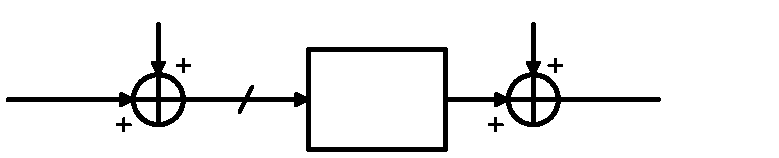
\includegraphics[scale=0.70000]{./figs/dco_noise.pdf}\\
   % translate x=-384 y=320 scale 0.38
   \putbox{1.02900in}{0.39200in}{0.96}{u[n]}%
   \putbox{1.48400in}{0.24500in}{0.96}{$\frac{2\pi K_{DCO}T}{1-z^{-1}}$}%
   \putbox{2.66700in}{0.34300in}{0.96}{$\Phi_{out}$[n]}%
   \putbox{0.78400in}{0.60900in}{0.96}{q$_{OTW}$[n]}%
   \putbox{0.18200in}{0.37800in}{0.96}{$\hat{\textnormal{u}}$[n]}%
   \putbox{2.54800in}{0.62300in}{0.96}{$\Phi_{n_{DCO}}$[n]}%
   } % close 'parbox'
   } % close 'scalebox'
   \vspace{-\baselineskip} % this is not necessary, but looks better
\fontfamily{\rmdefault}\selectfont

			\caption{ }
			\label{fig:dco_noise}
	    \end{subfigure}%
	    % \caption{Approximate model for ring oscillator inverter delay cell.}
	    \label{fig:osc_pn_figs}
	    \caption{\textbf{(a)} Leeson model for phase noise, \textbf{(b)} DCO additive noise model.}
	\end{figure}
	\FloatBarrier
	The equation for $\mathcal{L}(\Delta f)$ (from \cite{lee_hajimiri_2000}) is in \ref{eq:leesons}, and is dependent on the temperature T, excess noise factor F, oscillator power P, oscillator Q factor, and the transition frequencies $f_1$ and $f_2$ that separate the different noise regions. It is of interest to note that the phase noise relative to the carrier will increase as power decreases, which provides challenge for creating low power oscillators with acceptable phase noise characteristics.
	\begin{equation}\label{eq:leesons}
	\mathcal{L}(\Delta f) = 10\log_{10}\left[\frac{2\text{F}k_B\text{T}}{\text{P}}\left(1+\left(\frac{f_2}{2Q\Delta f}\right)^2\right)\left(1+\frac{f_1}{|\Delta f|}\right)\right] = S_{\Phi n_{DCO}}(\Delta f)
	\end{equation}
	For notational consistency, the following redefinition is used in the remainder of this paper: $S_{\Phi n_{DCO}}(f) = \mathcal{L}(\Delta f)|_{\Delta f = f}$

\subsubsection{Divider noise}
	\begin{figure}[htb!]
	    \centering
	    \begin{subfigure}{0.5\textwidth}
	        \centering
	        \fontfamily{\sfdefault}\selectfont
% XCircuit output "div_noise_model.tex" for LaTeX input from div_noise_model.ps
\def\putbox#1#2#3#4{\makebox[0.00000in][l]{\makebox[#1][l]{}\raisebox{\baselineskip}[0.00000in][0.00000in]{\raisebox{#2}[0.00000in][0.00000in]{\scalebox{#3}{#4}}}}}
\def\rightbox#1{\makebox[0.00000in][r]{#1}}
\def\centbox#1{\makebox[0.00000in]{#1}}
\def\topbox#1{\raisebox{-0.60\baselineskip}[0.00000in][0.00000in]{#1}}
\def\midbox#1{\raisebox{-0.20\baselineskip}[0.00000in][0.00000in]{#1}}
   \scalebox{1}{
   \normalsize
   \parbox{2.75260in}{
   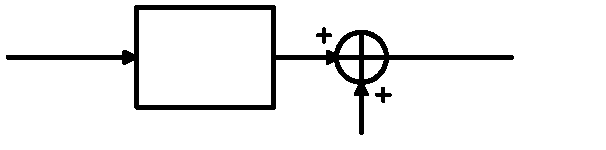
\includegraphics[scale=0.70000]{./figs/div_noise_model.pdf}\\
   % translate x=-96 y=524 scale 0.38
   \putbox{0.04200in}{0.53200in}{1.20}{$\Phi_{out}$[n]}%
   \putbox{0.79800in}{0.39200in}{1.20}{$\div \mathrm{N}$}%
   \putbox{1.74300in}{0.05600in}{1.20}{$\Phi_{n_{div}}$}%
   \putbox{1.84800in}{0.53200in}{1.20}{$\Phi_{div}$[n]}%
   } % close 'parbox'
   } % close 'scalebox'
   \vspace{-\baselineskip} % this is not necessary, but looks better
\fontfamily{\rmdefault}\selectfont

	        \caption{ }
	        \label{fig:div_pn_model}
	    \end{subfigure}%
	    \begin{subfigure}{0.5\textwidth}
	        \centering
	        \fontfamily{\sfdefault}\selectfont
% XCircuit output "div_jitter.tex" for LaTeX input from div_jitter.ps
\def\putbox#1#2#3#4{\makebox[0.00000in][l]{\makebox[#1][l]{}\raisebox{\baselineskip}[0.00000in][0.00000in]{\raisebox{#2}[0.00000in][0.00000in]{\scalebox{#3}{#4}}}}}
\def\rightbox#1{\makebox[0.00000in][r]{#1}}
\def\centbox#1{\makebox[0.00000in]{#1}}
\def\topbox#1{\raisebox{-0.60\baselineskip}[0.00000in][0.00000in]{#1}}
\def\midbox#1{\raisebox{-0.20\baselineskip}[0.00000in][0.00000in]{#1}}
   \scalebox{1}{
   \normalsize
   \parbox{2.61563in}{
   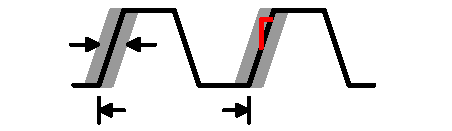
\includegraphics[scale=0.90000]{./figs/div_jitter.pdf}\\
   % translate x=-116 y=432 scale 0.38
   \putbox{0.80100in}{0.07200in}{1.20}{$\mathrm{N}/f_{osc}$}%
   \putbox{0.05400in}{0.61200in}{1.20}{$\sigma_{\Phi n_{div}}$}%
   \putbox{1.28700in}{0.59400in}{1.20}{$\frac{dV}{dt}$}%
   } % close 'parbox'
   } % close 'scalebox'
   \vspace{-\baselineskip} % this is not necessary, but looks better
\fontfamily{\rmdefault}\selectfont

	        \caption{ }
	        \label{fig:div_jitter}
	    \end{subfigure}
	    % \caption{Approximate model for ring oscillator inverter delay cell.}
	    \label{fig:div_pn}
	    \caption{\textbf{(a)} Divider noise model, \textbf{(b)} Digital divider output jitter.}
	\end{figure}
	\FloatBarrier
	Divider noise is manifested as jitter (with RMS distribution in time of $\sigma_{t n_{div}}$) on the divider output. If the divider is a digital circuit, with edge rate $dV/dt$, and subject to thermal noise in the form of an additive voltage $v_n$, with noise power of $\sigma_{v_n}^2$, the divider phase noise power added to the divider output is:
	\begin{equation}
		\sigma_{\Phi n_{div}}^2 = \omega^2_{ref}\sigma^2_{t n_{div}}  =\omega^2_{ref}\left(\frac{dV}{dt}\right)^{-2}\sigma_{v_n}^2
	\end{equation}
	At lock, the output of a digital divider will have an update rate $f_{{osc}}/\mathrm{N} \approx f_{ref}$, which can be treated as the sampling rate of the output phase signal $\Phi_{div}[n]$ as mentioned in section \ref{div_theory}. Thus if the divider phase noise power is confined into a bandwidth equal to $f_{ref}$, the spectral density of divider noise is:
	\begin{equation}
		S_{\Phi n_{div}}(f) = \frac{\sigma_{\Phi n_{div}}^2}{f_{ref}} = 2\pi\omega_{ref}\sigma^2_{t n_{div}}  =2\pi\omega_{ref}\left(\frac{dV}{dt}\right)^{-2}\sigma_{v_n}^2\hspace{1em}\frac{[\text{rad}]^2}{[\text{Hz}]}
	\end{equation}

\subsubsection{Loop filter noise - direct form I}\label{lf_noise}
	In a digital loop filter, quantization noise arises from rounding errors due to finite precision in the arithmetic circuits that implement the filter. Quantization noise power here will be derived under the assumption of a direct form I filter implementation, with B bits in each fixed point word throughout the loop filter. In a digital implementation of the canonical z-domain transfer function \ref{eq:canon_z_tf} as the direct form I structure of figure \ref{fig:direct_type_1_ideal}, delays are constructed using registers, adders with digital adders, and the filter coefficient gain terms $\{a_1, ... a_N; b_0, ..., b_M\}$ with digital multipliers. The registers and adders do not introduce extra round-off error beyond that already existing (if overflows do not occur). However, the multipliers will if the products resulting from two B bit words (nominally 2B bits), are mapped back onto B bit words.
	\begin{equation}
		\textnormal{H}_{LF}(z) = \frac{\sum_{j=0}^Z b_jz^{-j}}{1+\sum_{k=1}^P a_kz^{-k}}\label{eq:canon_z_tf}
	\end{equation}
	\FloatBarrier
	Quantization in this case can be represented by adding a quantization error signal $q_x$[n] to the result of each ideal multiplication, as shown in figure \ref{fig:direct_type_1_quant}. This is the same approach for TDC quantization noise in section \ref{tdc_noise}. The noise power associated with each q$_x$[n] is identical, with $\sigma_{qx}^2 = 1/12$ LSB$^2$. 

	\begin{figure}[htb!]
	    \centering
	    \begin{subfigure}{0.5\textwidth}
	        \centering
	        \fontfamily{\sfdefault}\selectfont
% XCircuit output "direct_type_1.tex" for LaTeX input from direct_type_1.ps
\def\putbox#1#2#3#4{\makebox[0.00000in][l]{\makebox[#1][l]{}\raisebox{\baselineskip}[0.00000in][0.00000in]{\raisebox{#2}[0.00000in][0.00000in]{\scalebox{#3}{#4}}}}}
\def\rightbox#1{\makebox[0.00000in][r]{#1}}
\def\centbox#1{\makebox[0.00000in]{#1}}
\def\topbox#1{\raisebox{-0.60\baselineskip}[0.00000in][0.00000in]{#1}}
\def\midbox#1{\raisebox{-0.20\baselineskip}[0.00000in][0.00000in]{#1}}
   \scalebox{1}{
   \normalsize
   \parbox{2.59948in}{
   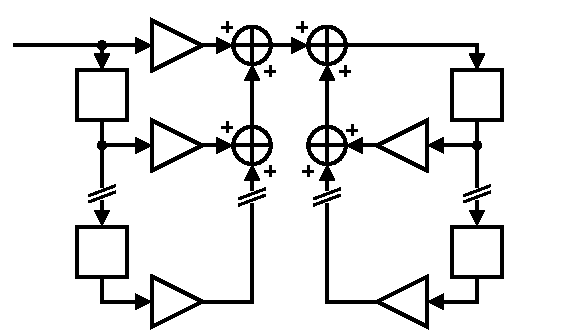
\includegraphics[scale=0.70000]{./figs/direct_type_1.pdf}\\
   % translate x=936 y=992 scale 0.38
   \putbox{0.04200in}{1.42800in}{0.96}{x[n]}%
   \putbox{2.28200in}{1.33700in}{0.96}{y[n]}%
   \putbox{0.37800in}{1.07800in}{0.96}{$z^{-1}$}%
   \putbox{0.84000in}{1.45600in}{0.96}{b$_0$}%
   \putbox{0.84000in}{0.98700in}{0.96}{b$_1$}%
   \putbox{2.12800in}{1.07800in}{0.96}{$z^{-1}$}%
   \putbox{2.12800in}{0.34300in}{0.96}{$z^{-1}$}%
   \putbox{1.71500in}{1.00100in}{0.96}{-a$_1$}%
   \putbox{1.70100in}{0.27300in}{0.96}{-a$_\mathrm{P}$}%
   \putbox{2.28200in}{0.86800in}{0.96}{y[n-1]}%
   \putbox{0.37800in}{0.34300in}{0.96}{$z^{-1}$}%
   \putbox{0.84000in}{0.25900in}{0.96}{b$_\mathrm{Z}$}%
   } % close 'parbox'
   } % close 'scalebox'
   \vspace{-\baselineskip} % this is not necessary, but looks better
\fontfamily{\rmdefault}\selectfont

	        \vspace{1.2em}
	        \caption{Ideal structure.}
	        \label{fig:direct_type_1_ideal}
	    \end{subfigure}%
	    \begin{subfigure}{0.5\textwidth}
	        \centering
	        \fontfamily{\sfdefault}\selectfont
% XCircuit output "direct_type_1_quant.tex" for LaTeX input from direct_type_1_quant.ps
\def\putbox#1#2#3#4{\makebox[0.00000in][l]{\makebox[#1][l]{}\raisebox{\baselineskip}[0.00000in][0.00000in]{\raisebox{#2}[0.00000in][0.00000in]{\scalebox{#3}{#4}}}}}
\def\rightbox#1{\makebox[0.00000in][r]{#1}}
\def\centbox#1{\makebox[0.00000in]{#1}}
\def\topbox#1{\raisebox{-0.60\baselineskip}[0.00000in][0.00000in]{#1}}
\def\midbox#1{\raisebox{-0.20\baselineskip}[0.00000in][0.00000in]{#1}}
   \scalebox{1}{
   \normalsize
   \parbox{2.92760in}{
   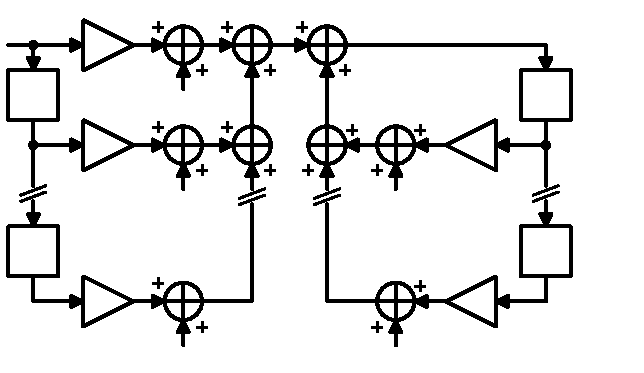
\includegraphics[scale=0.70000]{./figs/direct_type_1_quant.pdf}\\
   % translate x=936 y=1041 scale 0.38
   \putbox{0.05600in}{1.60300in}{0.96}{x[n]}%
   \putbox{2.60400in}{1.51900in}{0.96}{y[n]}%
   \putbox{0.05600in}{1.25300in}{0.96}{$z^{-1}$}%
   \putbox{0.51800in}{1.63100in}{0.96}{b$_0$}%
   \putbox{0.51800in}{1.16900in}{0.96}{b$_1$}%
   \putbox{2.44300in}{1.25300in}{0.96}{$z^{-1}$}%
   \putbox{2.44300in}{0.52500in}{0.96}{$z^{-1}$}%
   \putbox{2.03700in}{1.18300in}{0.96}{-a$_1$}%
   \putbox{2.02300in}{0.44800in}{0.96}{-a$_\mathrm{N}$}%
   \putbox{2.60400in}{1.05000in}{0.96}{y[n-1]}%
   \putbox{2.59000in}{0.32200in}{0.96}{y[n-2]}%
   \putbox{0.05600in}{0.52500in}{0.96}{$z^{-1}$}%
   \putbox{0.51800in}{0.43400in}{0.96}{b$_\mathrm{M}$}%
   \putbox{0.70700in}{1.25300in}{0.96}{q$_{b_0}$[n]}%
   \putbox{0.70700in}{0.78400in}{0.96}{q$_{b_1}$[n]}%
   \putbox{0.69300in}{0.05600in}{0.96}{q$_{b_\mathrm{M}}$[n]}%
   \putbox{1.68700in}{0.05600in}{0.96}{q$_{a_\mathrm{N}}$[n]}%
   \putbox{1.70100in}{0.78400in}{0.96}{q$_{a_1}$[n]}%
   } % close 'parbox'
   } % close 'scalebox'
   \vspace{-\baselineskip} % this is not necessary, but looks better
\fontfamily{\rmdefault}\selectfont

	        \caption{With added quantization error signals.}
	        \label{fig:direct_type_1_quant}
	    \end{subfigure}
	    % \caption{Approximate model for ring oscillator inverter delay cell.}
	    \label{fig:direct_type_1}
	    \caption{Direct form I filter implementation with quantization.}
	\end{figure}

	Assuming the quantization error signals of each multiplier are uncorrelated with all other multipliers, the output-referred noise power of the filter can be computed as the sum of the output-referred individual contributions. These contributions can be determined via solving for the transfer function from each source q$_x$[n] of each quantization noise to the output y[n]. In the case of the direct form I filter structure, all quantization sources q$_x$[n] have the same transfer characteristic to the output y[n] given in \ref{eq:lf_quant_tf}.
	\begin{equation}
		\frac{Y(z)}{Q_x(z)} = \frac{1}{1+\sum_{k=1}^P a_kz^{-k}}\label{eq:lf_quant_tf}
	\end{equation}
	Applying the bilinear transform to \ref{eq:lf_quant_tf}, with high oversampling where N$\cdot \text{BW}_{loop} 10 < f_{ref}$, and N is the number of poles in the system.
	\begin{equation}
		\left.\frac{Y(z)}{Q_x(z)}\right\vert_{z^{-1}=1-sT} \approx \frac{1}{1+\sum_{k=1}^P a_k - s\sum_{k=1}^P ka_k}\label{eq:lf_quant_tf_s}
	\end{equation}
	The output power spectral density is then for one error source is, confined to a bandwidth defined by the (sampling) reference frequency $f_{ref}$:
	\begin{equation}
		S_{qx}(f) = \frac{\sigma_{qx}^2}{f_{ref}}\left|\frac{Y(s)}{Q_x(s)}\right|^2_{s=j2\pi f} \approx \frac{1}{12f_{ref}}\left|\frac{1}{1+\sum_{k=1}^P a_k - j2\pi f\sum_{k=1}^P ka_k}\right|^2 \hspace{1em}\frac{[\text{LSB}]^2}{[\text{Hz}]}
	\end{equation}
	Given P poles and Z zeros in the filter, the total output quantization PSD of the filter is \ref{eq:lf_noise}. The total loop filter noise PSD linearly scales with the number of multipliers in the direct form I filter implementation.
	\begin{equation}
		S_{qn_{LF}}(f) = (P+Z+1)S_{qx}(f) \hspace{1em}\frac{[\text{LSB}]^2}{[\text{Hz}]}\label{eq:lf_noise}
	\end{equation}

\subsubsection{PLL noise sensitivity transfer functions}
	Having developed models for noise of generated by each PLL component, noise sensitivity transfer functions must be computer to refer each noise source to the PLL output in terms of phase. In the developed noise theory, thus far all noise sources have been modeled as additive phase components. The full system model illustrating this is in figure \ref{fig:full_pll_noise}.
	\begin{figure}[htb!]
		\center\fontfamily{\sfdefault}\selectfont
% XCircuit output "discrete_pll_full_noise.tex" for LaTeX input from discrete_pll_full_noise.ps
\def\putbox#1#2#3#4{\makebox[0.00000in][l]{\makebox[#1][l]{}\raisebox{\baselineskip}[0.00000in][0.00000in]{\raisebox{#2}[0.00000in][0.00000in]{\scalebox{#3}{#4}}}}}
\def\rightbox#1{\makebox[0.00000in][r]{#1}}
\def\centbox#1{\makebox[0.00000in]{#1}}
\def\topbox#1{\raisebox{-0.60\baselineskip}[0.00000in][0.00000in]{#1}}
\def\midbox#1{\raisebox{-0.20\baselineskip}[0.00000in][0.00000in]{#1}}
   \scalebox{1}{
   \normalsize
   \parbox{6.30000in}{
   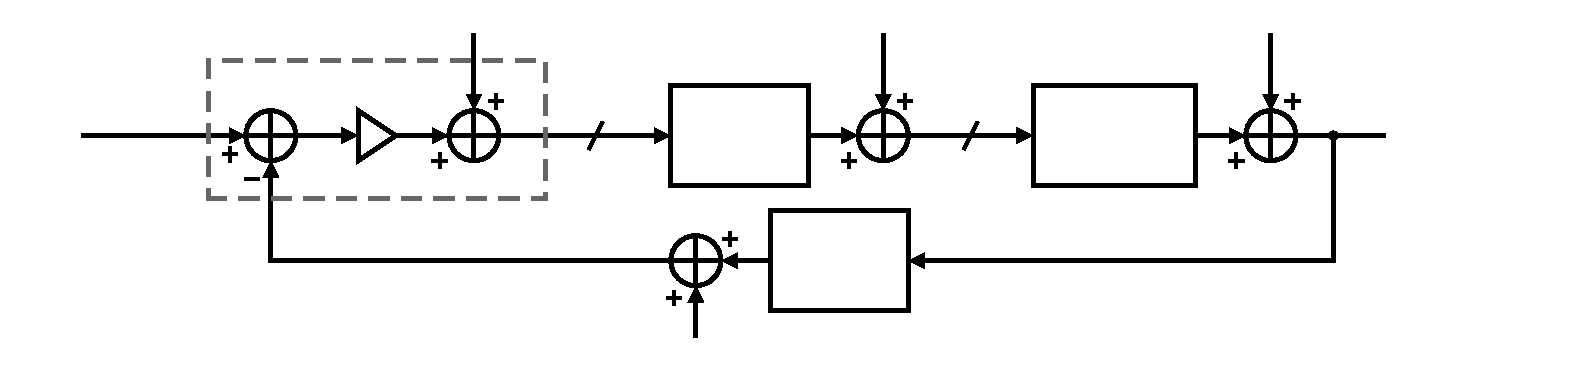
\includegraphics[scale=0.60000]{./figs/discrete_pll_full_noise.pdf}\\
   % translate x=416 y=544 scale 0.38
   \putbox{0.33600in}{1.00800in}{0.84}{$\Phi_{ref}$[n]}%
   \putbox{1.56000in}{0.52200in}{0.84}{$\Phi_{div}$[n]}%
   \putbox{2.27400in}{1.03200in}{0.84}{e$_\Phi$[n]}%
   \putbox{1.47000in}{1.07400in}{0.84}{\rotatebox{-360}{$\frac{\mathrm{M}}{2\pi}$}}%
   \putbox{1.20600in}{1.00800in}{0.84}{$\Phi_e$}%
   \putbox{0.83400in}{1.28400in}{0.84}{TDC}%
   \putbox{2.77200in}{0.89400in}{0.84}{H$_{LF}$(z)}%
   \putbox{3.79800in}{1.02000in}{0.84}{u[n]}%
   \putbox{4.22400in}{0.90600in}{0.84}{$\frac{2\pi K_{DCO}T}{1-z^{-1}}$}%
   \putbox{5.22000in}{0.99600in}{0.84}{$\Phi_{out}$[n]}%
   \putbox{3.22200in}{0.39600in}{0.84}{$\div$ N}%
   \putbox{4.13400in}{1.17000in}{0.84}{DCO}%
   \putbox{1.93200in}{1.30800in}{0.84}{q$_{n_{TDC}}$[n]}%
   \putbox{3.57000in}{1.30800in}{0.84}{q$_{n_{LF}}$[n]}%
   \putbox{2.82000in}{0.09600in}{0.84}{$\Phi_{n_{div}}$[n]}%
   \putbox{5.12400in}{1.30800in}{0.84}{$\Phi_{n_{DCO}}$[n]}%
   } % close 'parbox'
   } % close 'scalebox'
   \vspace{-\baselineskip} % this is not necessary, but looks better
\fontfamily{\rmdefault}\selectfont

		\caption{Full PLL additive noise model.}
		\label{fig:full_pll_noise}
	\end{figure}
	\FloatBarrier
	Following the approach of \cite{perrott_2002}, it is useful to define a transfer function $\hat{\mathrm{T}}(s)$ which characterizes the normalized closed loop response from reference to output of the PLL. $\hat{\mathrm{T}}(s)$ is defined in terms of the loop gain L(s).
	\begin{equation}
	\hat{\mathrm{T}}(s) = \frac{\mathrm{L}(s)}{1+\mathrm{L}(s)}\hspace{1em} \text{s.t.} \hspace{1em} \mathrm{T}(s) = \frac{\Phi_{out}}{\Phi_{ref}} = \mathrm{N}\hat{\mathrm{T}}(s) 
	\end{equation}
	Solving for the closed transfer functions between each $q_{n_{TDC}}$, $q_{n_{LF}}$, $\Phi_{n_{DCO}}$ and $\Phi_{n_{div}}$ to the output $\Phi_{out}$ utilizing s-domain approximations yields equations \ref{eq:noise_tf_tdc}-\ref{eq:noise_tf_div}.
	\begin{align}
		\frac{\Phi_{out}(s)}{q_{n_{TDC}}(s)} & = \frac{2\pi\frac{K_{DCO}}{s}\mathrm{H}_{LF}(s)}{1+\mathrm{L}(s)}= 2\pi\frac{\mathrm{N}}{\mathrm{M}}\frac{\mathrm{L}(s)}{1+\mathrm{L}(s)} = 2\pi\frac{\mathrm{N}}{\mathrm{M}}\hat{\mathrm{T}}(s)\label{eq:noise_tf_tdc}\\
		\frac{\Phi_{out}(s)}{\Phi_{n_{DCO}}(s)} & = \frac{1}{1+\mathrm{L}(s)}= 1-\hat{\mathrm{T}}(s)\\
		\frac{\Phi_{out}(s)}{q_{n_{LF}}(s)} & = \frac{2\pi\frac{K_{DCO}}{s}}{1+\mathrm{L}(s)} = 2\pi\frac{K_{DCO}}{s}(1-\hat{\mathrm{T}}(s))\\
		\frac{\Phi_{out}(s)}{\Phi_{n_{div}}(s)} & = \frac{\mathrm{M}\frac{K_{DCO}}{s}\mathrm{H}_{LF}(s)}{1+\mathrm{L}(s)}= \mathrm{N}\frac{\mathrm{L}(s)}{1+\mathrm{L}(s)} = \mathrm{N}\hat{\mathrm{T}}(s)\label{eq:noise_tf_div}
	\end{align}


\subsubsection{PLL phase signal and output PSD relationship for noise}\label{pn_noise_psd}
	When analyzing PLL noise, the noise power spectral density of the PLL output is of most interest. Up to this point, noise has been defined in terms of noise phase signal $\Phi_{n}$, or an unwanted added component to the oscillator phase signal $\Phi_{osc}=\omega_{osc}t$. The PLL output phase signal $\Phi_{out}$ is thus:
	\begin{equation}
		\Phi_{out}(t) = \Phi_{osc}(t) + \Phi_{n}(t) = \omega_{osc}t + \Phi_{n}(t) 
	\end{equation}
	Computation of PSD requires the PLL output voltage waveforms. These here will be defined in terms of complex exponentials. Given an oscillation amplitude $A_0$:
	\begin{equation}
		V_{out} = \Re\left(A_0e^{j\Phi_{out}(t)}\right) = \Re\left(A_0e^{j\omega_{osc}t}e^{j\Phi_{n}(t)}\right)
	\end{equation}
	Assuming the phase noise signal is zero mean, $\mathbb{E}[\Phi_{n}(t)]=0$, and the power of phase noise signal is small, $\mathrm{Var}[\Phi_{n}(t)] << 1$, then the approximation $e^{j\Phi_{n}(t)} = 1 + j\Phi_{n}(t)$ can be applied by truncating the exponential Taylor series expansion.
	\begin{align}
		V_{out} &= \Re\left(A_0e^{j\omega_{osc}t}e^{j\Phi_{n}(t)}\right) = \Re\left(A_0e^{j\omega_{osc}t} +j\Phi_{n}(t)A_0e^{j\omega_{osc}t}\right)\\
		&= A_0\cos(\omega_{osc}t) - \Phi_{n}(t)A_0\sin(\omega_{osc}t) \label{eq:pll_out_approx}
	\end{align}
	The result is a carrier cosine signal, and an orthogonal sine signal modulated by the phase noise $\Phi_{n}$. From this, the spectral density of the phase noise relative to the carrier can be estimated. The power spectral density $S_{V_{out}}$ is computed in \ref{eq:psd_vout}-\ref{eq:psd_noise}. Due to orthogonality of the sine/cosine components of \ref{eq:pll_out_approx}, the cross terms that appear in the PSD are zero. 
	\begin{align}
		S_{V_{out}}(f) =& \lim_{\Delta T\rightarrow\infty}\frac{1}{\Delta T}|\mathcal{F}\{V_{out}(t)\cdot\mathrm{rect}(t/\Delta T)\}|^2 \label{eq:psd_vout}\\
		=&\lim_{\Delta T\rightarrow\infty}\frac{A_0^2}{\Delta T}|\mathcal{F}\{\cos(\omega_{osc}t)\cdot\mathrm{rect}(t/\Delta T)\}|^2 \label{eq:psd_carrier}\\ 
		&+ \lim_{\Delta T\rightarrow\infty}\frac{A_0^2}{\Delta T}|\mathcal{F}\{\Phi_{n}(t)\cdot\mathrm{rect}(t/\Delta T)\}*\mathcal{F}\{\sin(\omega_{osc}t)\cdot\mathrm{rect}(t/\Delta T)\}|^2 \label{eq:psd_noise}
	\end{align}
	 The noise power spectral density $\mathcal{L}(\Delta f)$ is defined as the noise PSD at offset $\Delta f$ from the carrier frequency $f_{osc}$, normalized to the carrier power. Here the PSD carrier component is given by \ref{eq:psd_carrier}, and the noise component by \ref{eq:psd_noise}. Shifting \ref{eq:psd_noise} by $\omega_{osc}$ and performing normalization for carrier power results in:
	\begin{equation}\label{eq:pn_psd_relation}
		\mathcal{L}(\Delta f) = \left.\lim_{\Delta T\rightarrow\infty}\frac{1}{\Delta T}|\mathcal{F}\{\Phi_{n}(t)\cdot\mathrm{rect}(t/\Delta T)\}|^2 \right|_{f=\Delta f}= S_{\Phi_{n}}(\Delta f)
	\end{equation}

	Thus, the PLL output noise PSD relative to the carrier $\mathcal{L}(\Delta f)$ is equal to the PSD of the phase noise signal $\Phi_{n}(t)$, $S_{\Phi_{n}}(\Delta f)$, provided $\text{Var}[\Phi_{n}(t)] << 1$. 

\subsubsection{PLL output-referred noise PSD}\label{final_pn_model}
In terms of analysis, PLL noise PSD referred to the PLL output is of most interest. Thus far the following have been established: (a) noise spectrum generated by each individual PLL component, (b) the PLL phase noise sensitivity functions, and (c) the relationship between PLL output PSD and output phase noise. These can be combined to provide a final result for total PLL output-referred noise PSD. An assumption here is all noise sources are uncorrelated, so their independent noise power contributions may be summed to find the total noise PSD. The PLL output phase noise PSD for each noise source is simply found by multiplying magnitude squared of the respective noise sensitivity function with the noise source PSD. Thus:
\begin{align}
	S_{\Phi n_{TDC,out}}(f) &= S_{qn_{TDC}}(f)\left|\frac{\Phi_{out}(f)}{q_{n_{TDC}}(f)}\right|^2 = \frac{1}{12f_{ref}}\left|2\pi\frac{\mathrm{N}}{\mathrm{M}}\hat{\mathrm{T}}(f)\right|^2\\
	S_{\Phi n_{DCO,out}}(f) &= S_{\Phi n_{DCO}}(f)\left|\frac{\Phi_{out}(f)}{\Phi_{n_{DCO}}(f)}\right|^2  = \frac{S_{0\Phi n_{DCO}}}{f^2}\left|1-\hat{\mathrm{T}}(f)\right|^2\\		
	S_{\Phi n_{LF,out}}(f) &= S_{q n_{LF}}(f)\left|\frac{\Phi_{out}(f)}{q_{n_{LF}}(f)}\right|^2 \approx \frac{K_{DCO}^2}{12f_{ref}f^2}\frac{(P+Z+1)|1-\hat{\mathrm{T}}(f)|^2}{\left|1+\sum_{k=1}^P a_k - j2\pi f\sum_{k=1}^P ka_k\right|^2}\\
	S_{\Phi n_{div,out}}(f) &= S_{\Phi n_{div}}(f)\left|\frac{\Phi_{out}(f)}{\Phi_{n_{div}}(f)}\right|^2 = f_{ref}\left|2\pi\sigma_{tn_{div}}\mathrm{N}\hat{\mathrm{T}}(f)\right|^2
\end{align}
The output noise PSD at offset $\Delta f$ relative to the carrier normalized to carrier power of PLL will be:
\begin{equation}
	\mathcal{L}(\Delta f) = S_{\Phi n_{TDC,out}}(\Delta f) + S_{\Phi n_{DCO,out}}(\Delta f) + S_{\Phi n_{LF,out}}(\Delta f) + S_{\Phi n_{div,out}}(\Delta f)
\end{equation}

\subsection{Modified ADPLL architecture for low TDC resolutions}
When a low resolution TDC is used in a PLL, the resolution in phase will limit the ability to detect phase (or equivalently frequency) errors at the output in steady state. With M TDC steps per reference cycle, a divider ratio of N and a frequency error at the PLL output of $\Delta f$, the time needed for enough phase error to accumulate for a 1 LSB change of the TDC output is:
\begin{equation}
	t = \frac{\text{N}}{\text{M}\Delta f}
\end{equation}
If M $<$ N, the response time $t$ of the TDC to frequency disturbance $\Delta f$ is greater than the period of that disturbance $1/\Delta f$. Under these conditions, the PLL will have impaired ability to correct phase error and the phase noise performance will be degraded. In order to introduce higher resolution phase-feedback in steady state, a bang bang phase detector (BBPD) is added in parallel with the TDC, as in figure \ref{fig:bbpll}, weighted with a gain $K_{bb}$. The BBPD outputs a 1 if the divider signal is late relative to the clock, and -1 if it is early, with resolution limited only by jitter. Post the $K_{bb}$ gain, the power of the BBPD signal is $K_{bb}^2$. To ensure the noise generated by the BBPD is less than that expected for the TDC from quantization, $K_{bb}^2 < 1/12$.
\vspace{-1em}
\begin{figure}[htb!]
	\center\fontfamily{\sfdefault}\selectfont
% XCircuit output "bbpll.tex" for LaTeX input from bbpll.ps
\def\putbox#1#2#3#4{\makebox[0.00000in][l]{\makebox[#1][l]{}\raisebox{\baselineskip}[0.00000in][0.00000in]{\raisebox{#2}[0.00000in][0.00000in]{\scalebox{#3}{#4}}}}}
\def\rightbox#1{\makebox[0.00000in][r]{#1}}
\def\centbox#1{\makebox[0.00000in]{#1}}
\def\topbox#1{\raisebox{-0.60\baselineskip}[0.00000in][0.00000in]{#1}}
\def\midbox#1{\raisebox{-0.20\baselineskip}[0.00000in][0.00000in]{#1}}
   \scalebox{1}{
   \normalsize
   \parbox{3.33750in}{
   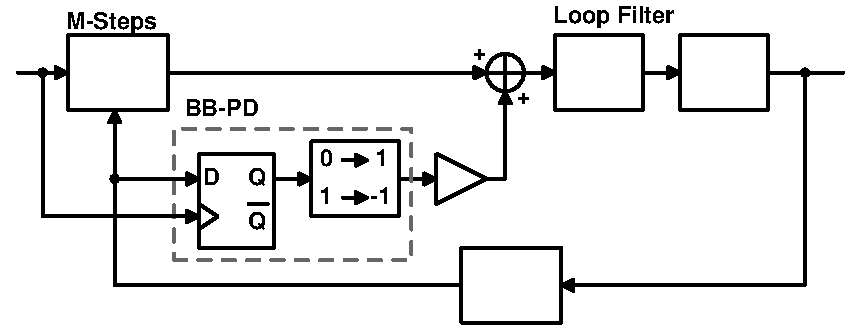
\includegraphics[scale=0.60000]{./figs/bbpll.pdf}\\
   % translate x=1412 y=528 scale 0.38
   \putbox{1.80600in}{0.70800in}{0.72}{$K_{bb}$}%
   \putbox{1.93200in}{0.14400in}{0.72}{$\div$ N}%
   \putbox{2.79600in}{0.99600in}{0.72}{DCO}%
   \putbox{2.24400in}{0.99600in}{0.72}{H$_{LF}$(z)}%
   \putbox{0.37200in}{0.99600in}{0.72}{TDC}%
   \putbox{0.03600in}{1.08600in}{0.72}{Clk}%
   \putbox{3.13200in}{1.08600in}{0.72}{Out}%
   } % close 'parbox'
   } % close 'scalebox'
   \vspace{-\baselineskip} % this is not necessary, but looks better
\fontfamily{\rmdefault}\selectfont

	\caption{PLL with parallel bang-bang phase detector and TDC.}
	\label{fig:bbpll}
\end{figure}
\FloatBarrier

% Out PSD = Noise PSD * |(TF from source to output)|^2

% out PSD = sum of individual PSDs

